\section {Methodology}

The approach to answering the research questions will be described in this section. The methodology consists of four parts. The first part describes the methods and literature that were used to select drugs and events. The second part describes the data pipeline which includes the data selection, data collection, data processing and data privacy. The third part describes the statistical metrics that were used to analyze the data. The last part covers the methods that were used to convey and visualize the data in the dashboard. 

\subsection {Drug and event selection methods}

\subsubsection {Method for drug selection}

To determine the different types of drugs which are used in the study, several institutes that collect data on drugs in the Netherlands were analyzed. The largest institution in the Netherlands that is related to drugs is the Trimbos Institute (TI). This national organization conducts research on the mental health of the Dutch people with a focus on the use of alcohol, tobacco and drugs. They involve all age groups in society and therefore cover the entire life cycle of citizens. This institute releases various analyses on alcohol, tobacco and other drug use in the Netherlands which includes reports on how to address these problems by naming prevention, education and policies. 

In addition, The TI tracks drug-related developments through various monitoring systems. The most important monitor is the National Drug Monitor (NDM). The NDM collects and compiles all data on substance use, the drug market and drug-related crime of all ages in the population. This institution aims to provide a representation of the figures known in the Netherlands related to drugs. Using both data from TI and NSM, a set of specific drugs were selected for this study. 


\subsubsection {Method for event selection}

First of all, it was determined which events would provide interesting results. Because of the sub-question "Which Dutch events are indicative for drug popularity?" it is interesting to use events where drug usage occurs a lot. Because where drugs are a popular means of enjoyment, they will also be used a lot.  For this purpose, research was done on the use of drugs at different events. That way, the events served as a proxy where drug usage is known to increase.
The first method that is used is literature research. This literary research was conducted to see if there has been previous research executed on drug use for different events in the Netherlands. 
However, very little is generally known about specific drug use per event in the Netherlands. Actually, there is no research done in the Netherlands about drug use at specific parties or events. Due to the fact that it is difficult to investigate because few drug users want to be open about their drug use. 
For that reason, we used another method where different news articles that say something about drug use per event are examined. This involves using different news sources, such as AD, NOS and Telegraaf, as well as regional news sources such as LokaalGelderland and Echt Amsterdams Nieuws. 
Using these two methods, a number of events have been identified where drugs are commonly used among the public. 

\subsection {Data methods}

\subsubsection{Data selection}
Before data could be collected and analyzed, a selection of data sources has been made. When it comes to the research question "To what extent can we identify event-based drug popularity on online data resources?", Google Trends data, Twitter data, and Dutch news data represent appropriate sources of information.

Google Trends data provides a comprehensive insight into the popularity of search terms and topics in real time. By analyzing the frequency of drug-related searches on Google, researchers can obtain a thorough understanding of drug popularity across regions and over time \cite{batistic}. Furthermore, Google Trends offers numerous filters and visualization options, making it a user-friendly tool for data analysis.

Twitter data represents a rich source of information on public
perceptions and opinions \cite{bian}. The platform is well known
for its user-generated content and real-time information, making
it a valuable resource for identifying the public's views on
drugs. Additionally, Twitter's hashtag and trending topic
features allow researchers to quickly identify the most popular
drug-related topics on the platform.

Dutch news data is a crucial source of information in the
assessment of event-based drug popularity. It provides a
comprehensive understanding of media representation of drug-
related events, including how these events are reported and
framed, and the public's perception of drug use. By analyzing
news data, researchers can gain a deeper insight into the
media's role in shaping public opinion on drug use \cite{mccombs}.

In conclusion, the combination of Google Trends, Twitter data, 
and Dutch news data offers a diverse and comprehensive set of 
data sources for understanding event-based drug popularity on
online data resources. These data sources provide valuable 
information on various aspects of drug use, such as search
trends, public opinion, and media representation, making them a
sound choice for answering the research question at hand.

\subsubsection{Data collection}

After data sources were selected, the data  was collected. The
Google Trends data was obtained using PyTrends, a library in
Python for accessing and retrieving data from Google Trends
\cite{PyPI}. This method of scraping allowed for an efficient
and automated process for collecting Google Trends data,
enabling the researcher to obtain a large amount of data in
short period. Only searches that were done on the territory of
The Netherlands were considered.

Twitter data was collected using SNscrape, a tool for scraping
social media data, including tweets and user profiles
\cite{GitHub}. This method of scraping Twitter data provided
access to a significant amount of real-time user-generated
content, allowing us to research the popularity of conversations
surrounding specific drugs in the Netherlands. We based on
Twitter scrape query on the time interval and keywords (e.g.
tweets between January 2014 - December 2022 that contained the
words ‘XTC’, ‘cocaine’ or ‘GHB’). Since we are only interested
in Dutch tweets, we excluded tweets that are non-Dutch. In
total, the Twitter scraper collected more than 1.500.000
relevant tweets.

 The Dutch news data was obtained by downloading a news corpus
 from the NOS, a Dutch public broadcaster. This method of data
 collection allowed us to access a large number of news articles
 in a centralized Kaggle repository, which was last updated at
 the end of 2022 \cite{Scheijen}. In total, the NOS contained
 more than 250.000 relevant news articles.

 \subsubsection{Data processing}

 After the selected data was collected datasets were loaded into
 a dataframe for processing. The pre-processing of the obtained
 Google Trends, Twitter, and Dutch news data was crucial in
 ensuring that the data was in a format suitable for analysis.
 To this end, the following pre-processing methods were applied:

\begin{itemize}
  \item Conversion of dates: All dates within the specified time
  frame were converted to the same datetime format. This
  standardization of the dates was essential for ensuring
  consistency in the data and making it easier to analyze.
  \item Calculation of week numbers: A function was created to
  calculate the week number of each date, as the time interval
  used for the analysis was "week." This function allowed for
  the grouping of data into weeks, making it easier to analyze
  trends and patterns over time.  The data was aggregated on a
  weekly level because that was the most granular aggregation of
  one of the sources \cite{GoogleTrends}. To have a comparative
  analysis, the weekly aggregation was applied to the data from
  all sources.
  \item Topic feature extraction: A function was created to
  check whether a tweet, news article, or search query contained
  a specific word, such as "cocaine" or "xtc." This process of
  topic feature extraction was essential in identifying and
  isolating the data that was relevant to the research question
  and in understanding the prevalence and significance of
  specific topics in the data.
  \item Normalization: The extracted features were normalized,
  as the values were absolute, while the Google Trends data were
  relative. Normalization between 0 and 100 was performed, and
  this came in useful when performing statistical tests and
  visualizing the data in the dashboard. Normalizing the data
  allowed for comparison and analysis of data from different
  sources, as the data were all expressed in the same unit.
\end{itemize}

\noindent Overall, the pre-processing of the Google Trends,
Twitter, and Dutch news data was essential in ensuring that the
data was in a suitable format for analysis. The conversion of
dates, calculation of week numbers, topic feature extraction,
and normalization was critical in making the data easier to
analyze and interpret, and in ensuring that the results obtained
from the analysis were accurate and reliable.

In addition, other pre-processing techniques such as sentiment
analysis, locational feature extraction, word2vec synonym
extraction and cleaning function have also been created. These
functions could be used in future work to extend the research,
make it more precise or compute detailed micro-level information.

\subsubsection{Data privacy}

In conducting the data collection and pre-processing of event
based drug popularity on online data resources, data privacy was
a significant consideration. All data sources used were
subjected to ethical and privacy considerations to ensure that
all personal information was protected and that the data was
collected, processed, and used in a responsible and ethical
manner.

It was ensured that all data sources used were publicly
available and did not contain any sensitive or personal
information. The Google trends data was collected via Pytrends,
in which personal information is already anonymized. For
example, Google Trends data did not contain any information on
the users who did the searches, but only the location where the
search happened. The Twitter data was obtained using the
SNscraper, which only collected data from public profiles and
ensured that the data collected did not contain any personal
information. For example, usernames and tags were removed.

In addition, appropriate measures were taken to protect the
privacy of individuals and organizations that provided the data.
For instance, all data was de-identified to remove any personal
information that could be used to identify individuals or
organizations.

\subsection {Statistical methods}

\subsubsection{Hypothesis}

To identify event-based drug popularity at events the following
hypothesis was formulated:
There is a significant increase in the metrics (number of
searches, -tweets and -news articles) of each data source during
the weeks of the events known for increased drug usage. 

\subsubsection{Computing peaks per regular week}

A metric was constructed in order to translate the hypothesis
into a test design. The data of each data source was aggregated
weekly to represent the counts per searches, tweets and news
articles respectively. 

The aggregated data was ordered chronologically and plotted on a
line plot. The peaks in the line plot were found using the
method signal. findpeaks from Pythons library Scipy \cite{scipy}. 
This step provided evidence on the weeks where there is an
increase in the representative metric in relation to the other
weeks in the considered time range (2014-2022). Figure \label{fig:peaks} is a representation of how the data was visualized after identifying the peaks of Google Trends searches.

\begin{figure}[h]
    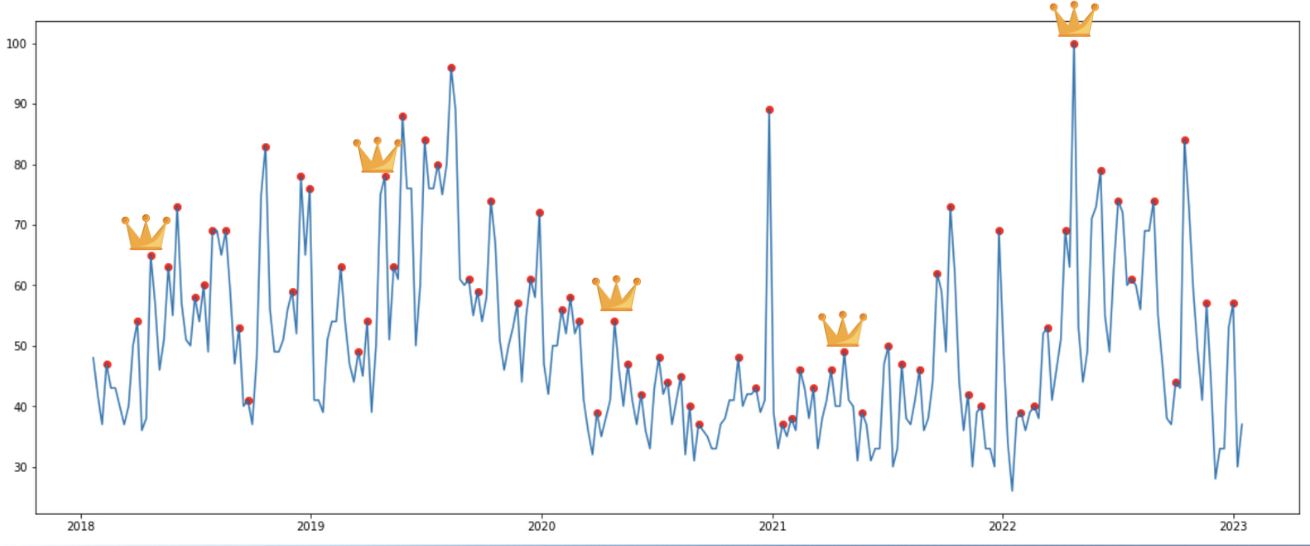
\includegraphics[width=3.25in]{peaks_over_years.png}
    \caption{}{King's day peaks per year}
    \label{fig:peaks}
\end{figure}

The data with labelled peaks was stored in a dataframe in the
form of a Bool column coupled with a column for the
corresponding week number. For instance if there was a peak in
Week 2 2022, the Bool column would be populated with True, else
it would be populated with False. With that each week number was
represented with 9 rows, 1 for each year between 2014 and 2022. 
Finally, a proportion was calculated for each week representing
the percentage of rows with “True” value out of the 9 rows for
each week. With that, each week was represented with a number
representing the percentage of years where a peak was observed
for that particular week.

\subsubsection{Computing peaks per event week}

The above steps were performed again in order to represent the
percentage of peaks for the weeks of the events with increased
drug usage (King’s day, ADE, Pride, Lowlands and New Year’s
Eve). This was needed because most of these events do not always
fall in the same week of the year.

For every year the dates of the events were identified. This was
necessary because some of the events happen on a different date
every year (e.g. ADE, Pride) \textit{appendix 1}. Based
on the event dates, the week in which each event happened was
identified \textit{appendix 1}. Based on the data extracted from the
line plot labelled with peaks, the years in which a peak
happened per week of the event were identified. Similarly, as in
the peaks per week, the percentage of weeks in which a peak was
observed was calculated.

\subsubsection{Test design}

A p-value approach proportion test was performed on the
generated data in order to test the hypothesis above
\cite{dialsingh}. The test was once for each combination of
drugs, events and data sources. Below are the specifications of
the test:

\begin{itemize}
  \item Null hypothesis (H0): The proportion of peaks observed
  in drug-related event weeks is not significantly larger than
  the proportion of peaks in regular weeks.
  \item Alternative hypothesis (H1): The proportion of peaks
  observed in drug-related event weeks is significantly larger
  than the proportion of peaks in regular weeks.
  \item Level of significance: To determine the level of
  significance, an alpha of 0.05 was used. This implies a 5\%
  risk of concluding that there is a larger proportion when
  there in reality that is not the case.
  \item Test statistic (z): The test statistic was calculated
  based on the sample proportion and population proportion, which is suitable for a proportion test. 
  \item Accepting the alternative hypothesis: The p-value was
  calculated from the test statistic. A p-value of less than
  0.05 (corresponding to the significance level) indicated
  evidence to reject the null hypothesis and accept the
  alternative hypothesis, and hence prove that the proportion of
  peaks during event weeks is indeed larger than regular weeks.

\end{itemize}

\subsection{Visualization methods}

\subsubsection{Dashboard}

One of the main objectives of the project was to produce a working prototype of a tool to map and visualize the data in a creative manner. It should adhere to basic visual and interaction design principles and standards allowing the analysts to analyse and interact with the data and explore the results of our research question.

After brainstorming and generated ideas it was decided to create a prototype of a dashboard where analysts would be able to see visual representations of the processed data and be able to interact with the interface to filter and compare the data to see interesting patterns and trends related to drug popularity. Further details of the look and feel and interaction of the dashboard is described in the \textit{results} chapter. Screenshots of the final dashboard are provided in \textit{appendix 1}

\subsubsection{User Requirements}

These user requirements are derived from the case description provided by the client as well as feedback from the stakeholder during the initial ideation and prototyping phase of the project and were further narrowed down during the project design workshops using the MoSCoW prioritization method. The term 'user' in the requirements refers to two specific types of similar target audiences that will make use of our prototype, police agents who want to explore the dataset to gain insights and data analysts who want to filter and compare our datasets.

 \begin{enumerate}
   \item (M) The user must be able to use the prototype on a personal computer and interface with a screen
   \item (M) The user must be able to filter the datasets to compare different years of data
   \item (M) The user must be able to filter the datasets to compare different types of drugs
   \item (M) The user must be able to overlay multiple datasets and trend lines on top of each other
   \item (M) The system uses open-source software and not locked-in corporate data tools
   \item (M) The system has a user-friendly visual design and interaction design
   \item (S) The user should create an account to store specific and personalized filters
   \item (S) The user should be able to download the raw datasets in specific file formats
   \item (S) The user should be able to navigate between different overviews showing corresponding data
   \item (C) The user could upload their own dataset and sources of specific drugs and news sources
   \item (C) The system uses real-time up-to-date API data
 \end{enumerate}

 \subsection{Collaboration methods}
